% -*- coding: UTF-8 -*-
\documentclass{article}
\usepackage{amsmath}
\usepackage{tikz}

\begin{document}
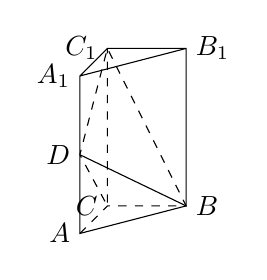
\begin{tikzpicture}

  \coordinate[label=180:$A$] (a) at (-0.35,-0.35);
  \coordinate[label=0:$B$] (b) at (1,0);
  \coordinate[label=180:$C$] (c) at (0,0);
  \coordinate[label=180:$A_1$] (a1) at (-0.35,1.65);
  \coordinate[label=0:$B_1$] (b1) at (1,2);
  \coordinate[label=180:$C_1$] (c1) at (0,2);
  \coordinate[label=180:$D$] (d) at (-0.35,0.65);

  \draw (d) -- (b) -- (b1) -- (c1) -- (a1) -- (a) -- (b) (a1) -- (b1);
  \draw[dashed] (a) -- (c) -- (b) -- (c1) -- (d) -- (c) -- (c1);

\end{tikzpicture}
\end{document}